\chapter{Initial Requirements}

\section{Introduction}
In this project we will create a SDN controller for defense against DDoS attacks. Through a REST API system, a web server can notify the begin of a DDoS attack: the controller will create an address change mechanism from D to D’ while filtering malicious clients.

Web Server will cooperate changing the listening address to a new one (called D') while opening another instance of the web server on the old address (called D). On this instance, however, the server will provide a forwarding mechanism to D' enough complex to not be executed by bots.
All used addresses are took from a list of addresses, which can be configurated through the controller REST APIs.

Filtering is made by counting the number of connections made by the client after the defence is enabled: if this count gets above a certain threshold, then the client is marked as a bot. However this behavior happens only if bots/clients don't use HTTP \textit{keep-alive} mode, which would be surreal and not praticable for performance reasons: to solve this, the forwarding HTTP server instance will cut the connection after sending the forwarding response.

\section{Implementation}
Any of the mentioned sources will be declared as part of \textbf{ddosdefence} package.

\subsection{Controller receive()}
In this project we will implement the controller code following the already provided pseudo code:
\begin{figure}[H]
\begin{center}
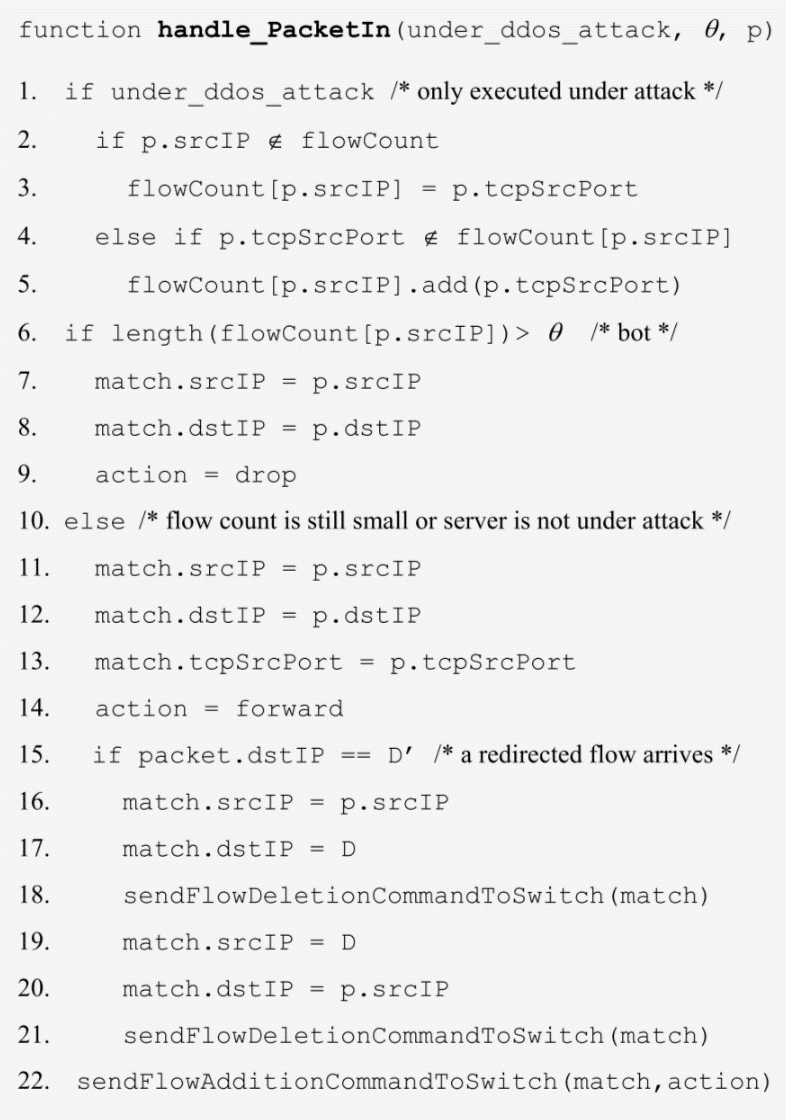
\includegraphics[width=0.8\textwidth]{images/PseudoCode.png}
\label{fig:pseudocode}
\caption{Controller pseudo code}
\end{center}
\end{figure}

\textit{flowCount} will be implemented using an HashMap where the key is the client source IP and the value a list of ports: however, to give an efficient implementation, we will use an Hash, this time an HashSet, also to implement each list of ports. This is due to the fact that searching is an operation often needed for both the lists.

The source name will be \textbf{DDoSDefence.java}.

\subsection{REST APIs}
At least two resources are needed to let the server manage and enable the service.

\subsubsection{DDoSDefend Initialization}
\textit{Address: /ddosdefence/init/json\\
Request Type: JSON, Response Type: empty or error\\\\}
Required to initialize the controller. Can be executed \textbf{only once}, as a simplification.
Values to be initialized are:
\begin{itemize}
	\item Service port: port binded by the service to defend
	\item Public Address pool: addresses used and sent back by controller when protection is enabled
	\item Threshold: max number of connection after client is marked as a bot
\end{itemize}

\begin{lstlisting}[caption={DDoSDefend Initialization Request format/example},captionpos=b]
	{
		serviceport: <valid port number>
		addresses: [pool of addresses]
		threshold: <valid natural number>
	}
\end{lstlisting}

In case of invalid parameter values, returns an error as Reponse Code.

\subsubsection{DDoSDefend Management}
\textit{Address: /ddosdefence/manage/json\\
Request Type: JSON, Response Type: IPv4 Address (string)\\\\}

Can be used to enable or disable the protection. When enabled, response is set to the new address on which the HTTP server must bind. When disabled, response is set to an empty string. Can be executed only \textbf{after Initialization}.

\begin{lstlisting}[caption={DDoSDefend Management Request format/example},captionpos=b]
	{
		enabled: <true/false>
	}
\end{lstlisting}

The source names will be \textbf{InitDefenceResource.java, EnableDefenceResource.java, IDDoSDefenceREST.java}.

\subsection{LearningSwitch module changes}
LearningSwitch provides an implementation of L2 switch autolearning and gives a thread-safe service interface to access the switching table. LearningSwitch provides a public method to get the port associated to a destination MAC Address, however this is not provided by the \textbf{ILearningSwitch} interface.
We will add the method to the interface, also assuming that we can execute it without any concurrency issue: this has been checked inspecting internal method implementation.

\section{Assumptions}
Before starting the project we have thought about the issues we would have met, so we made the following assumptions:

\subsubsection{Controller behavior}
\begin{itemize}
	\item Using OpenFlow \textgreater  1.3 for needed features
	\item Number of IP addresses: predefined and sufficient for the purpose of the project. IPs will be allocated using a circular list. We mainly assume that no client connects on \(D\) if server enabled the protection for more than one time (for example when it starts using \(D''\))
	\item ARP and ICMP Handling
		\begin{itemize}
			\item Will be done as a normal L2 switch would do
			\item Will be delegated to a modified version of LearningSwitch Floodlight module, which will autolearn mac/ports switching rules. This feature will be used by DDoSDefence module to implement the NORMAL forward action.
		\end{itemize}
\end{itemize}

\subsubsection{WebServer Behavior}
\begin{itemize}
	\item Our project requires implementing a CAPTCHA system. Due to the complexity and to the eventually required external connection made by this components, we will give a simplified implementation. A custom implementation is also required to let the client scripts to follow a CAPTCHA forward without human intervention (more in Testing chapter). \textbf{*}
	\item WebServer always reset/close a connection while sending a forwarding response. Required to manage keep-alive issues caused when client reuses the same source port for multiple requests (client connection count would not increase).
	\item WebServer must be always available, at least while protection is enabled, to not let clients make new connections due to timeout expiration.
	\item WebServer never initialize a connection. Simplifies response packet switch flow management.
\end{itemize}

\subsubsection{Testing needs}
\begin{itemize}
	\item REST interfacing will be done from the test machine and not from the virtualized hosts. This is due to the issues that would create when a virtual host wants to connect to the external controller
	\item WebServer will be emulated using a Python script and not an usual implementation. \textbf{*}
\end{itemize}

\textbf{*} could be modified according to the difficulties encountered during implementation.

\section{Testing System}
Our module will be tested using a set of scripts that we will produce. Mininet APIs will be used to create a virtual network composed by:
\begin{itemize}
	\item One server;
	\item A fixed number of clients (mixed Bot and Users).
\end{itemize}

Server (h1) can use addresses from a /24 subnet, in our case 7.7.7.0/24 will be used.
Each client (h2-hN) will use an addresses took from the 80.80.80.0/24 subnet.

The Controller will listen for OpenFlow PACKET\_IN connections on 127.0.0.1:6653.
One OpenFlow switch (s1) will be used to connect all the previous entities.

\begin{figure}[H]
\begin{center}
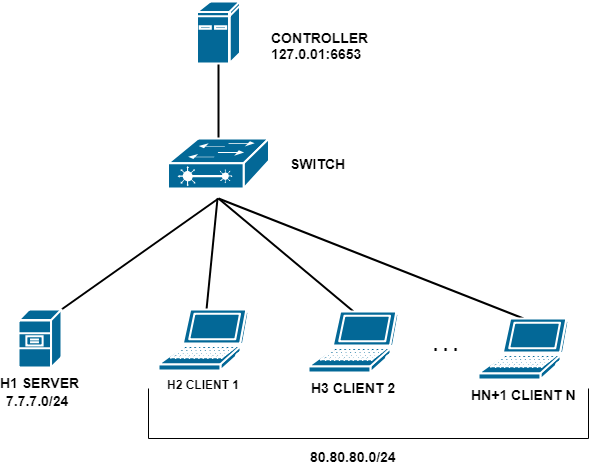
\includegraphics[width=0.8\textwidth]{images/TestingTopology.png}
\label{fig:testing}
\caption{Testing Topology}
\end{center}
\end{figure}

No routing or complex forwarding rules are required because the switch will solve the problem only using L2 Table packet switching. The only rule to use on both server and clients is \\
\begin{lstlisting}
route add -net 0.0.0.0/32 dev <out interface>
\end{lstlisting}

to send all the packet originated from the emulated device through the interface connected to the switch. ARP mechanism on the packet originating device will make sure to set the correct destination MAC address.
Clients can be regular service users or malicious ones:
\begin{itemize}
	\item Bots: will continuously do HTTP requests to a single target, but will not be able to compute any complex forwarding (like CAPTCHA or JavaScript execution),
	\item Clients: will perform regular HTTP requests and be able to do forwarding.
\end{itemize}	
Both behaviours will be simulated using two separate scripts. Pseudo-code examples could be:
\paragraph{./start\_bot.sh serverip}
Start one connection at time and retry to connect if disconnected, with no end. Bots behavior can be different than this, for example another one bot could start more connection asynchronusly. However this would just increase the connection count of system and could be implemented just using more synchronous bots.
\begin{lstlisting}[caption={./start\_bot.sh pseudo code},captionpos=b]
while(true) {
	Establish HTTP on server connection using keepalive;
	retry when connection is closed
}
\end{lstlisting}

\paragraph{./start\_client.sh serverip}\
\begin{lstlisting}[caption={./start\_client.sh pseudo code},captionpos=b]
while(true) {
	Establish HTTP on server connection on serverip using keepalive;
	continue when connection is closed
	serverip = (if forwarded)  ? newaddress : serverip ; # user can follow forward
	print forwarded address if forwarded
	sleep 2; # user will generate less traffic than bots
}

\end{lstlisting}

As stated on the paper, the forwarding method must be sufficiently complex to not be executed by the bots. However this represents an issue for ./start\_client.sh script that is, in reality, a bot itself. To overcome this issue, we can initially simplify the forwarding mechanism to let the script do the forward. However the ./start\_bot.sh will ignore, in good faith, the simplified forwarding directive.

An example of HTTP Page forwarding response could be one not containing an HTML page (we can check if contains \textless html\textgreater\ or not) but containing the address to forward. This is just for a testing purpose and can be subjected to changes as a consequence of chosen web server implementation.

\subsubsection{Checking the correct behaviour for OpenFlow rules:}
This command can be used to dump flow entries of all switches.
\begin{lstlisting}
mininet> dpctl dump-flows
\end{lstlisting}

This will be used to check if controller behavior follows the requirements. The following tests can be done:

\paragraph{BOT/Client Connections arriving when protection is OFF}
Every connection/packet must be forwarded to the server and every (response) packet generated from server must be forwarded to client. This means we expect a list of entries like this:
\begin{lstlisting}
<<ARP Entries>>
src=<client ip>:<port>, dst_ip=<D>:<listen port>, ACTION: FORWARD
src=<srv_ip>:<listen port>, dst_ip=<cl_ip>:<cl_port>, ACTION: FORWARD
\end{lstlisting}

\paragraph{BOT Connections arriving when protection is ON}
We expect the same result as before, until client connections becomes more than threshold. At this point we expect (assuming only 1 connection made by client after threshold):
\begin{lstlisting}
<<ARP Entries>>
<<Old FORWARD Entries for connections started before reaching thresh.>>
src=<client ip>:<port>, dst_ip=<D>:<listen port>, ACTION: DROP
\end{lstlisting}
Old forward entries will be cleared by a rule timeout. Note that the web server, when forwarding, closes the connection after responding to the request, so, after the server response, all the Forward rules are not matched anymore.

\paragraph{Client Connections arriving when protection is ON}
If the client connects to D' address, all the old forward/drop rules related to that client must be deleted. So, after a client connects to D', we expect:
\begin{lstlisting}
<<ARP Entries>>
src=<client ip>:<port>, dst_ip=<D'>:<listen port>, ACTION: FORWARD
\end{lstlisting}
No old rules must be found.

%\subsubsection{Testing Parameters}
%%%%%DA SISTEMARE%%%%
%Timeout ? (quello nel codice di anto)
%\tehta = attack flow entry count threshold
%Cmax = number of maximum allowable connections
%Cattack = number of attack signaling connections
%n = number of legitimate users
%k = number of  bots
%\lamba norm - average request arrival rate from legitimate users
%\lamba attack - average request arrival rate from bots
%\mu service rate

\section{Final Documentation and Reporting}
At the end of this project will be produced:
\begin{itemize}
	\item Final report: accompanying document illustrating the choices made and the reasons for these choices for the implementation of the module,
	\item Summary presentation in which the work carried out will be shown,
	\item Demo to show how the module works.
\end{itemize}
